\chapter[Experiments]{Experiments} Validation encompasses the
entire methodology in how analysis on models are performed. \citet{Sargent2004}
categorized a large number of methods into a concise list. The list is not
limited to a specific science domain or type of model, and when describing
validation used in a research paper, a link can usually be made back to
Sargent's list. Because the goal of understanding all information available
about validation is large, it is typically researched in smaller and more
specific pieces such that over time the information gained from the research
will make it easier to understand validation as a whole.

The next three sections describe validation experiments that were performed to
gain a better understanding of space weather models. Three magnetosphere models
were studied using a less utilized, but important, validation method than that
more commonly found in the space weather literature. In the first section, the
responses of magnetospheric MHD models to a common space weather phenomenon that
is linked to causing harmful effects on space-based technology is considered.
This phenomena is a change in the z direction of the magnetic field in the
upstream solar wind from positive to negative. In the second section, the
effect of differences in preconditioning times for MHD magnetospheric models is
analyzed. In the last section, the effects of two extreme space weather
conditions on the MHD magnetospheric models is considered. First, conditions in
space weather that cause high magnetospheric compression are analyzed and then
conditions that cause low magnetospheric compression are considered. In all
analyses, a tool specifically developed for this research, called model output
difference imaging, is used to visualize the differences between model outputs.

\section[IMF $B_z$ Reversal]{Response to a reversal in $B_z^{IMF}$
from positive to negative}

\subsection{Background}
The first research done on the impact in the magnetosphere of a southward
directed interplanetary magnetic field ($B_s$) was in the late 1960's and early
1970's when the Dungey theory of magnetospheric convection was tested. The
support for Dungey's claim came from positive correlations between the AE geomagnetic index and the
magnitude of $B_s$ \citep{Maezawa1976}. \citet{Gonzalez2005} analyzed 64 intense
geomagnetic storms and showed that the time delay between the
peak $B_s$ and the minimum $D_{st}$ value was approximately two hours. \citet{Gonzalez2005}
noted that because the typical storm duration was approximately ten hours for
the storms studied, the two hour delay can represent up to 20\% of the main
phase of a typical storm. This is important to forecasters as they can use this
information to predict that the minimum $D_{st}$ will occur, on average, two
hours after peak $B_s$.

Analysis was done on the interplanetary conditions that caused
geomagnetic storms during solar cycle 23 \citep{Echer2008}. One
of the conclusions was that out of the 90 storm events considered, none
of them occurred during northward IMF. They also found that the structures that
led to the intense southward IMF, ordered from highest to lowest occurrence
frequency, were magnetic clouds, sheath fields, combined magnetic cloud and
sheath fields, and co-rotating interaction regions.

\subsection{Motivation}
There are many factors involved in the response of the magnetosphere to the
solar wind. Numerous studies have been performed to offer
explanations on why certain space weather events occur, and they have been
tested with strong statistical support. To better understand how a change in a single variable effects the
magnetospheric system, as approximated by MHD models, it was decided to perform
a \textit{parameter variability - sensitivity analysis} validation in which the
only changing parameter was $B_z^{IMF}$, which changed from positive to negative.
In this analysis, the other input variables ($B_x^{IMF}$, $B_y^{IMF}$,
$\mathbf{V}$, $\rho$, and $T$) were kept constant to limit the number of
factors that may influence model output and to simplify
interpretation.

\subsection{Methodology}
\label{SimilarMethodology}
When comparing two models through visual inspection of each output separately,
there is difficulty involved in determining what the major differences between
the two are. The motivation for developing a model output differencing
visualization tool was to make this type of comparison easier. First, data from
each of the MHD magnetospheric models  was placed and interpolated onto one
common grid. An open source tool, Kameleon (\textit{Kameleon}, 2013), developed by the CCMC, was used for
the interpolation. Kameleon is a C++ based code that
supports a few of the available CCMC MHD magnetospheric models. The Kameleon software supports the OpenGGCM, BATS-R-US, and
SWMF models, which are the three MHD magnetospheric models used in these
experiments. Finally, a tool was needed that could load a large data set, plot
all of it, and view planar cuts. The tool used for this was
Paraview (\textit{Paraview}, 2013) which is maintained by Kitware
(\textit{Kitware}, 2013), Paraview was specifically designed to enable 3-D
visualization of scientific data and to handle very large data sets with
parallelized operations. Paraview also has a Python interface, which
allows plots to be made and manipulated via a script instead of manually using
a graphical user interface.

The second tool was used for the \textit{parameter variability - sensitivity
validation} analysis \citep{Sargent2004}. This technique was implemented by
inputting artificial data into magnetospheric MHD models, that are not in-situ
based, in order to make controlled comparisons between model outputs. All of the
data used as input into the models are of this form.

There are many magnetospheric models, and because the time required to make a
comparison between them is prohibitive, and given the limitation of the
Kameleon library, which at present only supports three magnetospheric MHD
models, three MHD magnetospheric models were chosen for the experiments.
To work around the limits of compiling and executing the models, the
models were executed on computers at the CCMC.

\subsubsection{Acquiring Data}
\begin{figure}
	\centering
	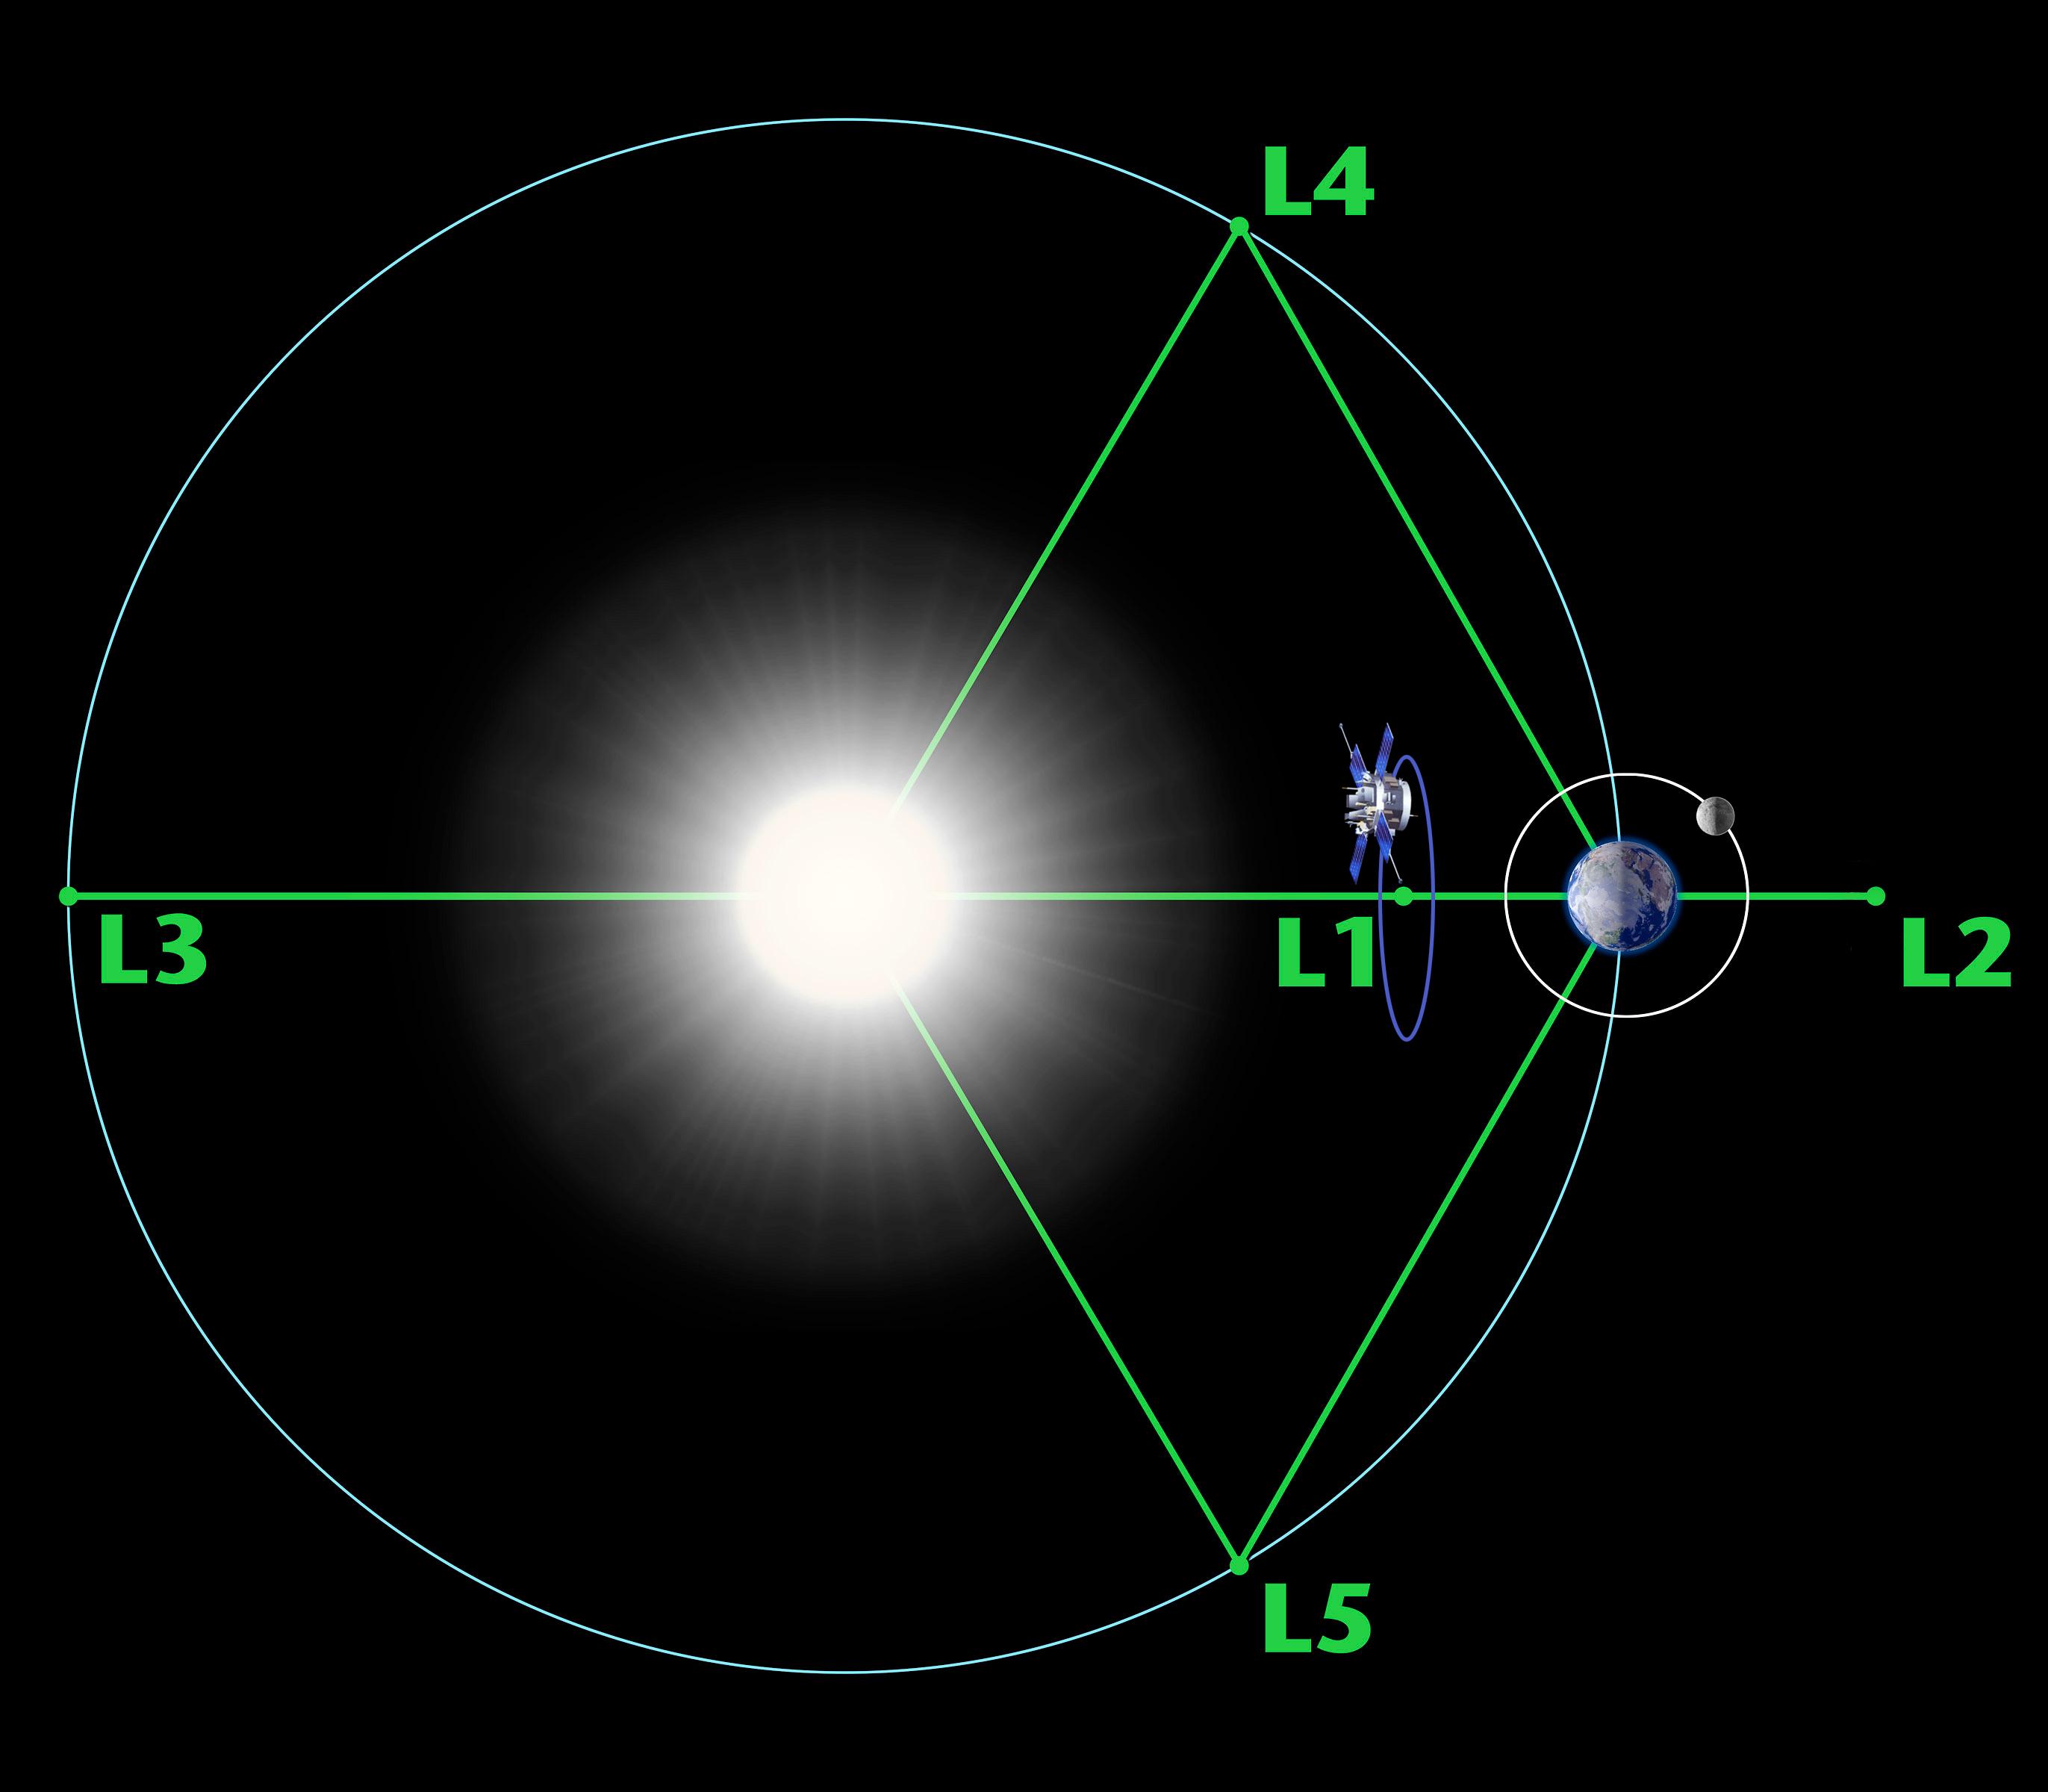
\includegraphics[scale=0.1]{images/LagrangePoints.jpg}
	\caption{The five Lagrange points (from NASA, \citeyear{Lagrange}).}
    \label{fig:LagrangePoints}
	\figSpace
\end{figure}
The uniqueness to the \textit{parameter variability} technique described previously is
that the data used as inputs into the models are not in-situ measurements from
the past, but are physically relevant artificial data that has meaning to the
space weather community. The CCMC allows for model runs to be configured using a
web interface; the run is submitted to staff who then execute the
model with the selected inputs and configuration. The input parameters are
submitted through a data file that contains values for $\mathbf{B^{IMF}}$,
$\mathbf{V}$, $\rho$, $T$. To determine the values to use as artificial inputs,
Advanced Composition Explorer (ACE) measurements were used because they
provide measurements from the solar wind taken from the L1 point ahead of Earth
in the Sun-to-Earth line over a full solar cycle, as shown in Figure
\ref{fig:LagrangePoints}. The in-situ data that was measured by instruments on
the ACE spacecraft were obtained from the OMNIWeb web site provided by the NASA
Goddard Space Flight Center (OMNIWeb, \citeyear{OMNIWeb}) between the dates of
January 1st, 2000 to January 1st, 2011.

\begin{figure}
	\centering
	\subfigure[Mean = 5.76 $cm^{-3}$, 80th and 20th Percentile = 11/2 $cm^{-3}$,
	95,128 Measurements]{
		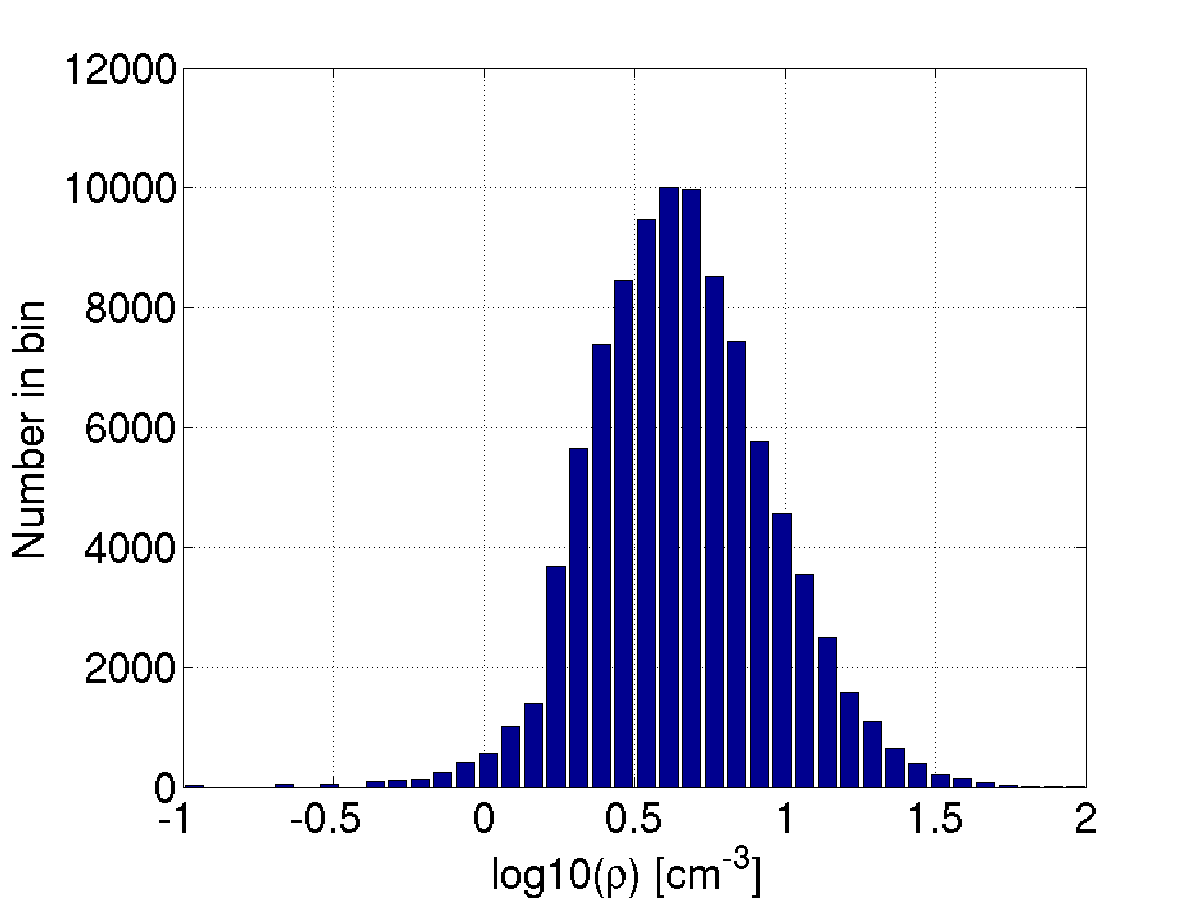
\includegraphics[scale=0.35]{images/hist_N.png}
	    \label{fig:hist_n}
	}\quad
	\subfigure[Mean = 101289 $K$, 80th and 20th Percentile = 217139/20554 $K$,
	95,255 Measurements]{
		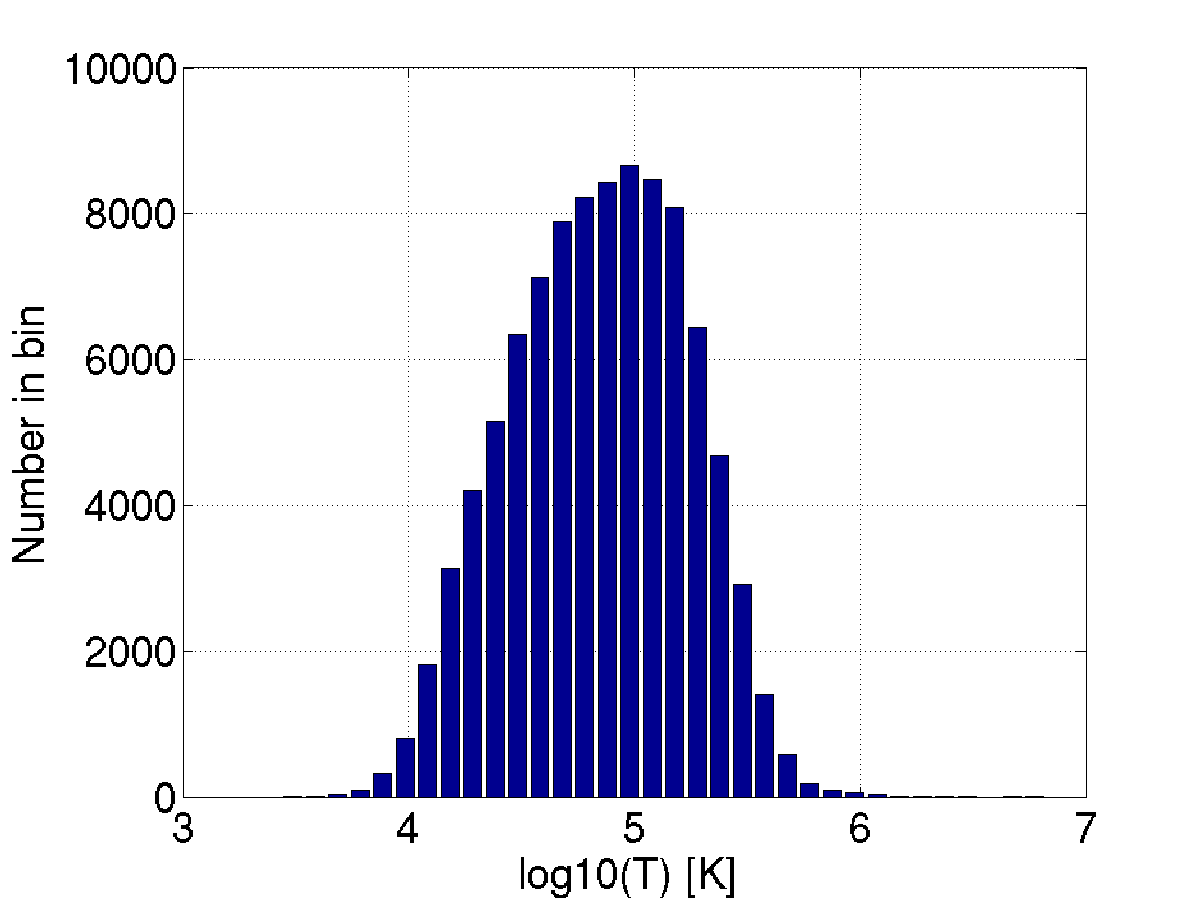
\includegraphics[scale=0.35]{images/hist_T.png}
	    \label{fig:hist_t}
	}\\
	\subfigure[Mean = 0.02 $nT$, 80th and 20th Percentile = 3.1/-3.0 $nT$, 96,417
	Measurements]{
		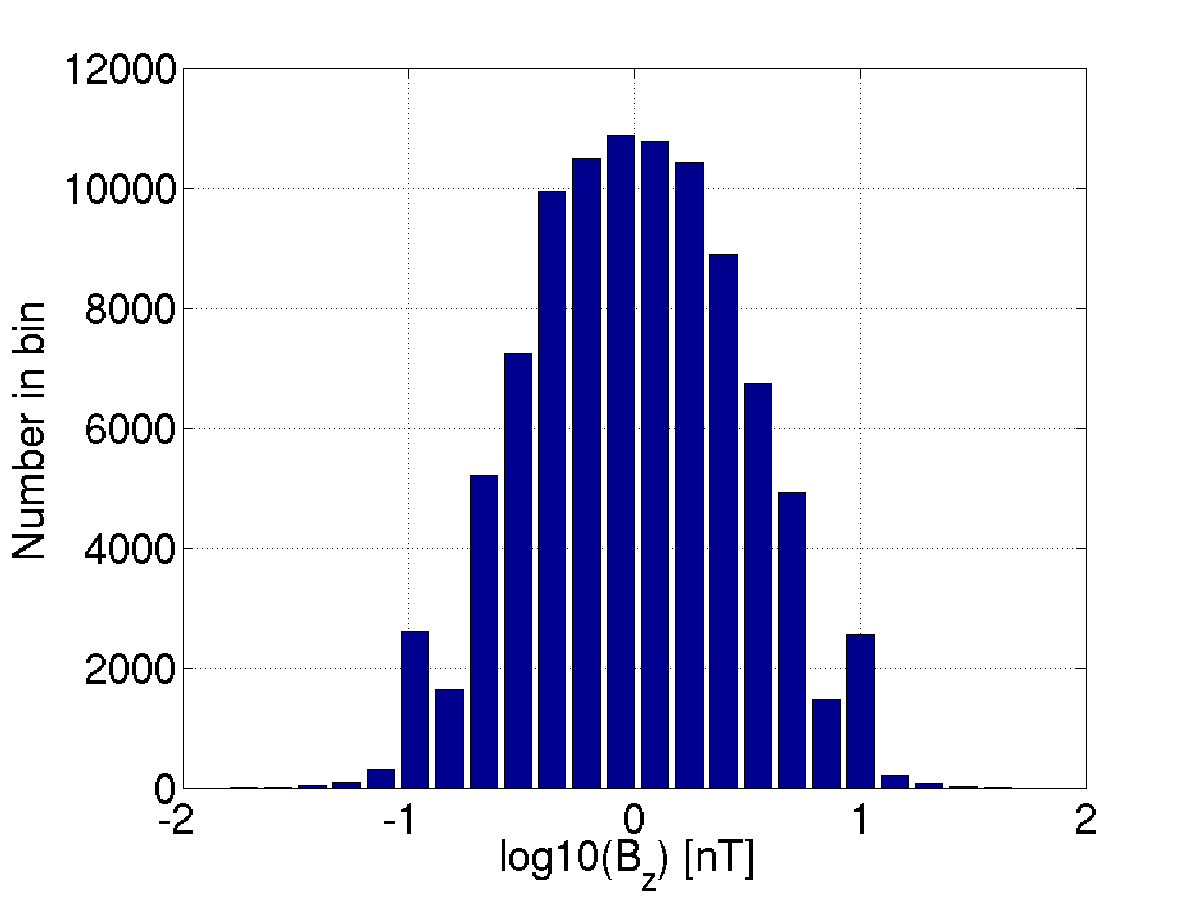
\includegraphics[scale=0.35]{images/hist_BZ.png}
	    \label{fig:hist_bz}
	}\quad
	\subfigure[Mean = 441.71 $km/s$, 80th and 20th Percentile = 604/320 $km/s$,
	96,311 Measurements]{
		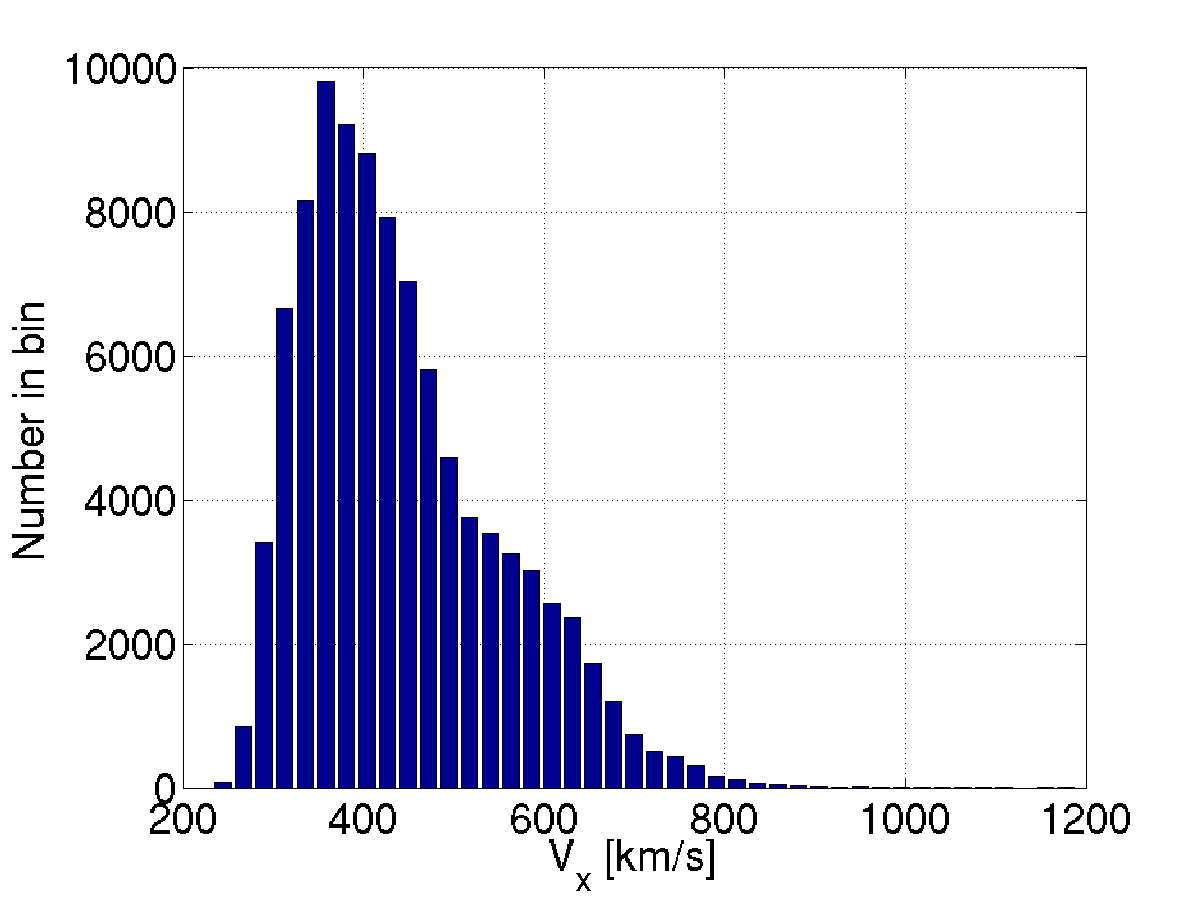
\includegraphics[scale=0.35]{images/hist_V.png}
	    \label{fig:hist_v}
    }
    \caption{Histogram of (a) $\rho$, (b) $T$, (c) $B_z^{IMF}$ and (d) $V_x$
    values measured by ACE, from January 1st, 2000 to January 1st, 2011. These
    histograms were used to determine appropriate values as artificial inputs to the models.}
	\figSpace
\end{figure}

MATLAB was used to read in the OMNIWeb data files, and histograms were created
for the solar wind variables. Figure \ref{fig:hist_n} is the histogram of solar
wind plasma density. The mean is 5.76 [$cm^{-3}$], the 80th percentile is 11
[$cm^{-3}$], and the 20th percentile is 2 [$cm^{-3}$]. Figure \ref{fig:hist_t}
is the histogram of solar wind temperature. The mean is 101289 [$K$], the 80th
percentile is 217139 [$K$] and the 20th percentile is 20554 [$K$]. Figure
\ref{fig:hist_bz} is the histogram of the solar wind interplanetary magnetic
field. The mean is 0.02 [$nT$], the 80th percentile is 3.1 [$nT$] and the 20th
percentile is -3.0 [$nT$]. Figure \ref{fig:hist_v} is the histogram of solar
wind velocity in the x direction, from Earth towards the Sun. The mean is 442 [$km/s$], the 80th percentile is 604 [$km/s$]
and the 20th percentile is 310 [$km/s$]. The 20th and 80th percentiles were used
for consistency with climatological values from in-situ data, specifically for
the experiment studying the effects of extreme solar wind conditions on the magnetosphere, higher and lower values for input
conditions are required to simulate high and low compression.
The percentile and mean values for each variable are displayed in Table
\ref{table:histtable}.

\begin{table}
\begin{center}
  \caption{ACE solar wind measurement histograms}
  \begin{tabular}{| l | c | c | c | }
    \hline
    \textbf{Variable} & \textbf{20th Percentile} & \textbf{Mean} &
    \textbf{80th Percentile} \\
    \hline $\rho$ [$cm^{-3}$] & 2 & 5.76  & 11   \\ \hline
    $T$ [$K$] & 20554 & 101289  & 217139 \\ \hline
    $V_x$ [$km/s$] & 310 & 442 & 604 \\ \hline
    $B_z$ [$nT$] & -3.0 & 0.02 & 3.1 \\ \hline
  \end{tabular}
  \label{table:histtable}
\end{center}
\end{table}

The simulations analyzed in this section used the input values shown in Table
\ref{table:run1}.

\begin{table}
\begin{center}
  \caption{Input parameters for $B_z^{IMF}$ reversal experiment}
  \begin{tabular}{| l | c | c | c | c | }
    \hline
    \textbf{$\rho$} [$cm^{-3}$] & \textbf{$T$} [$K$] &
    \textbf{$V_x$} [$km/s$] &
    \textbf{$B_z$} [$nT$]
    \\
    \hline 
    5.76 & 101289 & -442  & +3.1 to -3.0 at 00:30 \\ \hline
  \end{tabular}
  \label{table:run1}
\end{center}
\end{table}

\subsection{Results}

There are two different time periods in each run where the overall state of the
magnetosphere will significantly differ. First, the period of time before the
$B_z^{IMF}$ reversal occurs in which the magnetic field of the IMF is the same
direction as Earth's. Second, the period of time after the $B_z^{IMF}$ reversal
in which the direction of the IMF is opposite to that of Earth's. The reversal in $B_z^{IMF}$ occurs 30 minutes into each
run, the total time for each run was 6 hours. The changes expected are only due
to a reversal in $B_z^{IMF}$ direction and the differences between each model.

The grid used in the OpenGGCM model is different than that used in the BATS-R-US and SWMF models.
The stretched cartesian grid used in the OpenGGCM model has high resolutions in the
entire current sheet region and high resolutions near-Earth extending in the
Z and Y directions from the origin. The SAMR grid used in the BATS-R-US and SWMF models
has high resolution near-Earth and in the near-Earth current sheet region with
lower resolutions in the distant tail and distant northern and southern tail
lobes.

There are differences in how each model treats magnetospheric conditions
near-Earth (within 10$R_E$). The OpenGGCM and BATS-R-US models do not account
for particle drifts associated with the ring current. The SWMF model accounts
for particle drifts and the ring current.

The differences between the BATS-R-US and SWMF models are expected to be due to
the ring current. Based on Ampere's law, $\nabla \times \mathbf{B} =
\mu_0 \mathbf{J}$, the additions of a ring current should lead to an increase
of the z component of the magnetic field on the sunward side of the ring current
and decrease the z component of the magnetic field on the tailward side of
the ring current. This means the magnetic pressure is expected to be larger in
the sunward side of the ring current and smaller in the tailward side of the
ring current.

The magnetic pressure at the dayside magnetopause is effected by the reversal
from a positive $B_z^{IMF}$ direction to a negative $B_z^{IMF}$ direction. A
decrease in the magnetic pressure at that location will cause a movement of the
magnetopause towards Earth.

Figure \ref{fig:OpenGGCMatReversal} shows the OpenGGCM model output during the timeframe
where the magnetopause moves Earthward due
to a reduction in magnetic pressure, consistent with expectations. 
\begin{figure}
	\centering
	\subfigure{%
		\includegraphics[scale=0.36]{/mnt/Disk2/Brian_Curtis_042213_1/Results/images/Bz_File8.png}
		}
	\subfigure{%
		\includegraphics[scale=0.36]{/mnt/Disk2/Brian_Curtis_042213_1/Results/images/Bz_File9.png}
		}
	\subfigure{%
		\includegraphics[scale=0.36]{/mnt/Disk2/Brian_Curtis_042213_1/Results/images/Bz_File10.png}
		}
	\caption{OpenGGCM $B_z$ output shortly after the $B_z^{IMF}$ reversal.}
	\figSpace
	\label{fig:OpenGGCMatReversal}
\end{figure}

To better understand the differences in the position of the magnetopause
between the three models before and after the $B_z^{IMF}$ reversal,
model output difference images are used.

Figure \ref{fig:BdiffBeforeFlip} shows three comparisons between two models at a
time. The top image is a percent difference of $B_z$ between the OpenGGCM and
BATS-R-US models; the BATS-R-US model values are subtracted from the OpenGGCM model
values for each grid point on the interpolated grid and that result is
divided by their mean at that grid point. The middle image is a percent difference of $B_z$ between
the OpenGGCM and SWMF models. The bottom image is a percent difference of $B_z$
between the BATS-R-US and SWMF models. The top image of Figure \ref{fig:BdiffBeforeFlip}
shows large and negative percent differences near the location of the magnetopause. The negative value means that the second model in the top image, BATS-R-US, has
higher values. From this type of information, the model with the farthest and
closest magnetopause can be determined. Before the $B_z^{IMF}$ reversal the OpenGGCM model
magnetopause is closest to Earth and the SWMF model magnetopause is farthest
from Earth.
\begin{figure}
	\centering
	\subfigure{
		\includegraphics[scale=0.36]{/mnt/Disk2/Results/0_1/images/Bz_Diff_File1.png}
		}
	\subfigure{
		\includegraphics[scale=0.36]{/mnt/Disk2/Results/0_2/images/Bz_Diff_File1.png}
		}
	\subfigure{
		\includegraphics[scale=0.36]{/mnt/Disk2/Results/1_2/images/Bz_Diff_File1.png}
		}
	\caption{$B_z$ percent differences between the OpenGGCM and
	BATS-R-US models (top), the OpenGGCM and SWMF models (middle), and the BATS-R-US
	and SWMF models (bottom) 25 minutes before the $B_z^{IMF}$ reversal.}
	\figSpace
	\label{fig:BdiffBeforeFlip}
\end{figure}

The SWMF model has a slightly higher magnetic pressure near the magnetopause in
comparison to the BATS-R-US model, which can be explained by the effect that the ring
current has locally. The differences in current strength before the $B_z^{IMF}$
reversal are shown in Figure \ref{fig:JxRingCurrent}, where comparing the top
(BATS-R-US) and bottom (SWMF) images, the tail currents are lower with the SWMF
model. Earth has a ring current brought about by the motions of plasma
trapped in the near-Earth magnetosphere. This current, which lies between
4-7 $R_E$, induces its own magnetic field. The direction of its magnetic field 
in the near-Earth tail region opposes the direction of the field created by the current
sheet current, weakening it near-Earth. The direction of $B_z$ from the ring
current near the magnetopause is the same as the direction of Earth's magnetic
field and thus increases the magnetic pressure in that location. That increase
in magnetic pressure explains why the SWMF model magnetopause is farthest from
Earth, as shown in Figure \ref{fig:BdiffBeforeFlip}.

\begin{figure}
	\centering
	\subfigure{%
		\includegraphics[scale=0.36]{/mnt/Disk2/Brian_Curtis_042213_2/Results/images/Jx_File1.png}
		}
	\subfigure{%
		\includegraphics[scale=0.36]{/mnt/Disk2/Brian_Curtis_042213_3/Results/images/Jx_File1.png}
		}
	\caption{$J_x$ for BATS-R-US (top) and SWMF (bottom).}
	\figSpace
	\label{fig:JxRingCurrent}
\end{figure}

Figure \ref{fig:BdiffAfterFlip}, 60 minutes after the $B_z^{IMF}$ reversal, shows that
under negative $B_z^{IMF}$ conditions, the OpenGGCM model magnetopause is closest to
Earth and the BATS-R-US magnetopause is farthest from Earth.

\begin{figure}
	\centering
	\subfigure{
		\includegraphics[scale=0.36]{/mnt/Disk2/Results/0_1/images/Bz_Diff_File30.png}
		}
	\subfigure{
		\includegraphics[scale=0.36]{/mnt/Disk2/Results/0_2/images/Bz_Diff_File30.png}
		}
	\subfigure{
		\includegraphics[scale=0.36]{/mnt/Disk2/Results/1_2/images/Bz_Diff_File30.png}
		}
	\caption{$B_z$ Percent differences between the OpenGGCM and
	BATS-R-US models (top), the OpenGGCM and SWMF models (middle), and the
	BATS-R-US and SWMF models (bottom) 60 minutes after the $B_z^{IMF}$ reversal.}
	\figSpace
	\label{fig:BdiffAfterFlip}
\end{figure}

When plasma from the sun traveling at supersonic speeds interacts with the
magnetosphere, it eventually slows down below the speed of sound. This
transition from supersonic to subsonic causes a shock region ahead of the
magnetosphere, which is referred to as the bow shock. The velocity of the plasma
continues to decrease as it compresses and heats, leading to higher densities
between the magnetopause and the bow shock. Figure \ref{fig:rhoBeforeFlip} shows
this for all three models. There are higher densities in the current sheet that
are typically on the order of 0.1 to 1 $cm^{-3}$, but these values fit
in one color bin of the plots and are not visible.

Through various mechanisms, plasma can enter the magnetosphere cavity. Some of this plasma becomes
trapped on the closed magnetic field lines that surround Earth resulting in higher near-Earth densities.
The differences in densities seen near-Earth and in the tail region
between the models before the $B_z^{IMF}$ reversal are shown in Figure
\ref{fig:rhodiffBeforeFlip}. The larger differences seen in the magnetotail when
comparing the OpenGGCM model with the SWMF model
is due to the OpenGGCM model not accounting for the ring current. This
plot also shows that the SWMF model has highest densities in the current sheet
region.

\begin{figure}
	\centering
	\subfigure{%
		\includegraphics[scale=0.36]{/mnt/Disk2/Brian_Curtis_042213_1/Results/images/rho_File1.png}
		}
	\subfigure{%
		\includegraphics[scale=0.36]{/mnt/Disk2/Brian_Curtis_042213_2/Results/images/rho_File1.png}
		}
	\subfigure{%
		\includegraphics[scale=0.36]{/mnt/Disk2/Brian_Curtis_042213_3/Results/images/rho_File1.png}
		}
	\caption{$\rho$ for OpenGGCM (top) , BATS-R-US (middle), and SWMF (bottom) 25
	minutes before the $B_z^{IMF}$ reversal.}
	\figSpace
	\label{fig:rhoBeforeFlip}
\end{figure}

\begin{figure}
	\centering
	\subfigure{
		\includegraphics[scale=0.36]{/mnt/Disk2/Results/0_1/images/rho_Diff_File1.png}
		}
	\subfigure{
		\includegraphics[scale=0.36]{/mnt/Disk2/Results/0_2/images/rho_Diff_File1.png}
		}
	\subfigure{
		\includegraphics[scale=0.36]{/mnt/Disk2/Results/1_2/images/rho_Diff_File1.png}
		}
	\caption{$\rho$ Percent differences between the OpenGGCM and
	the BATS-R-US models (top), the OpenGGCM and SWMF models (middle), and the
	BATS-R-US and SWMF models (bottom) 25 minutes before the $B_z^{IMF}$ reversal.}
	\figSpace
	\label{fig:rhodiffBeforeFlip}
\end{figure}

After the $B_z^{IMF}$ reversal, shown in Figure \ref{fig:rhodiffAfterFlip}, the
OpenGGCM densities in the distant current sheet become higher than the
BATS-R-US. The SWMF model still has higher densities in the current sheet, which
is shown in the third image that compares the BATS-R-US and SWMF models (where
there are darker blue colors in the current sheet).

\begin{figure}
	\centering
	\subfigure{
		\includegraphics[scale=0.36]{/mnt/Disk2/Results/0_1/images/rho_Diff_File45.png}
		}
	\subfigure{
		\includegraphics[scale=0.36]{/mnt/Disk2/Results/0_2/images/rho_Diff_File45.png}
		}
	\subfigure{
		\includegraphics[scale=0.36]{/mnt/Disk2/Results/1_2/images/rho_Diff_File45.png}
		}
	\caption{$\rho$ Percent differences between the OpenGGCM and
	BATS-R-US models (top), the OpenGGCM and SWMF models (middle), and the
	BATS-R-US and SWMF models (bottom) 115 minutes after the $B_z^{IMF}$ reversal.}
	\figSpace
	\label{fig:rhodiffAfterFlip}
\end{figure}

As noted previously, and shown in Figure \ref{fig:UxBeforeFlip}, the solar wind
$U_x$ slows down from a supersonic to a subsonic speed which causes a shock.
$U_x$ is then reduced more as its distance from Earth decreases.
The current sheet is formed from two opposing magnetic field directions close to
one another, which is caused by the stretching in the
magnetotail. In this region there is a near-zero $B_z$, which allows for
reconnection. This reconnection transports particles in the current sheet region
both tailward and Earthward. The velocities seen in the current sheet region in
all models are consistent with this.
\begin{figure}
	\centering
	\subfigure{%
		\includegraphics[scale=0.36]{/mnt/Disk2/Brian_Curtis_042213_1/Results/images/Ux_File1.png}
		}
	\subfigure{%
		\includegraphics[scale=0.36]{/mnt/Disk2/Brian_Curtis_042213_2/Results/images/Ux_File1.png}
		}
	\subfigure{%
		\includegraphics[scale=0.36]{/mnt/Disk2/Brian_Curtis_042213_3/Results/images/Ux_File1.png}
		}
	\caption{$U_x$ for OpenGGCM (top), BATS-R-US (middle), and SWMF (bottom) 25
	minutes before the $B_z^{IMF}$ reversal.}
	\figSpace
	\label{fig:UxBeforeFlip}
\end{figure}

Before the $B_z^{IMF}$ reversal, Figure \ref{fig:UxdiffBeforeFlip} shows that the
OpenGGCM model has higher $U_x$ in the distant tail current sheet compared to
the BATS-R-US model and the SWMF model. The near-Earth current sheet velocities
are higher in the BATS-R-US model and the SWMF model than the OpenGGCM model. In
comparison, the BATS-R-US model and the SWMF model comparison (bottom), shows
that the SWMF model has higher $U_x$ in the near-Earth current sheet and the
BATS-R-US model has higher $U_x$ in the distant tail.
\begin{figure}
	\centering
	\subfigure{
		\includegraphics[scale=0.36]{/mnt/Disk2/Results/0_1/images/Ux_Diff_File1.png}
		}
	\subfigure{
		\includegraphics[scale=0.36]{/mnt/Disk2/Results/0_2/images/Ux_Diff_File1.png}
		}
	\subfigure{
		\includegraphics[scale=0.36]{/mnt/Disk2/Results/1_2/images/Ux_Diff_File1.png}
		}
	\caption{$U_x$ percent differences between OpenGGCM and
	BATS-R-US (top), OpenGGCM and SWMF (middle), and BATS-R-US and SWMF (bottom)
	25 minutes before the $B_z^{IMF}$ reversal.}
	\figSpace
	\label{fig:UxdiffBeforeFlip}
\end{figure}

After the $B_z^{IMF}$ reversal, Figure \ref{fig:UxdiffAfterFlip} shows the
BATS-R-US model has higher $U_x$ compared to the OpenGGCM model in the current
sheet region (top), while the OpenGGCM model compared to the SWMF model (middle)
shows higher $U_x$ in the current sheet region for the OpenGGCM model and higher
$U_x$ in the north and south tail lobes outside of the current sheet region for
the SWMF model. Comparing the BATS-R-US model and the SWMF model (bottom), the
BATS-R-US model has higher $U_x$ in the current sheet region.
\begin{figure}
	\centering
	\subfigure{
		\includegraphics[scale=0.36]{/mnt/Disk2/Results/0_1/images/Ux_Diff_File31.png}
		}
	\subfigure{
		\includegraphics[scale=0.36]{/mnt/Disk2/Results/0_2/images/Ux_Diff_File31.png}
		}
	\subfigure{
		\includegraphics[scale=0.36]{/mnt/Disk2/Results/1_2/images/Ux_Diff_File31.png}
		}
	\caption{$U_x$ percent differences between OpenGGCM and
	BATS-R-US (top), OpenGGCM and SWMF (middle), and BATS-R-US and SWMF (bottom)
	85 minutes after the $B_z^{IMF}$ reversal.}
	\figSpace
	\label{fig:UxdiffAfterFlip}
\end{figure}

\subsection{Discussion and Conclusions}

The position of the magnetopause and shape of the magnetosphere are
determined by the magnetic field of Earth and its interaction with the
solar wind. The OpenGGCM model, which did not account for a
near-Earth ring-current, has the weakest magnetic pressure and therefore the
closest magnetopause to Earth of the three models. The model-predicted position
of the magnetopause is important for forecasters because they need to be able to tell companies with
space-based technologies, especially those in geosynchronous orbit, if their
equipment may be effected by the plasma that comes from the solar
wind.

\cite{Garcia2007} discuss how the absence of the ring current in the Lyon
Fedder Mobarry (LFM) magnetospheric model compares to magnetopause location
measurements made by satellites. They found that an insufficient ring current would not push the
magnetopause far enough Sunward. The ring current effect on the magnetopause
location is evident with this experiment as well.

The models show the slowdown of $U_x$ Earthward of the
bow shock, and inside the magnetosphere. The velocities in the current sheet
region are important to forecasters as to the timing of storms impacts seen at
Earth. Reconnection is tied to the
$U_x$ such that a faster reconnection will yield faster velocities and a slower
reconnection will yield slower velocities.

Model output differences can give model developers a better view of
the differences between their model and other models for similar regions in
space. With model runs involving in-situ data, the space weather community is
already doing a lot of analysis into determining which model is better for
select events.

\subsubsection{Summary}
For a reversal in $B_z^{IMF}$, the
following occur in the models:
\begin{itemize}
  \item The OpenGGCM model magnetopause is closest to Earth as it has the weakest
  near-Earth magnetic pressure.
  \item Under positive $B_z^{IMF}$ conditions, the ring current pushes the SWMF
  model magnetopause farther sunward than that in the BATS-R-US model.
  \item Under negative $B_z^{IMF}$ conditions, the SWMF model magnetopause is
  farther Earthward than that in the BATS-R-US model.
  \item The differences in magnetopause positions between BATS-R-US and SWMF
  are due to the effects of the ring current addition to the SWMF model.
  \item Densities are highest with the SWMF model and lowest with the OpenGGCM
  model.
  \item The OpenGGCM model tail currents are significantly different from the
  BATS-R-US model and SWMF at over 100 percent differences.
\end{itemize}

